\subsection{Macrobenchmarks}
\label{macro}

%%%%%%%%%%using figures to present incast: tput, fariness, droprate, TCP RTT
\begin{figure}[!t]
        \centering
        \begin{subfigure}[b]{0.45\textwidth}
                \centering
                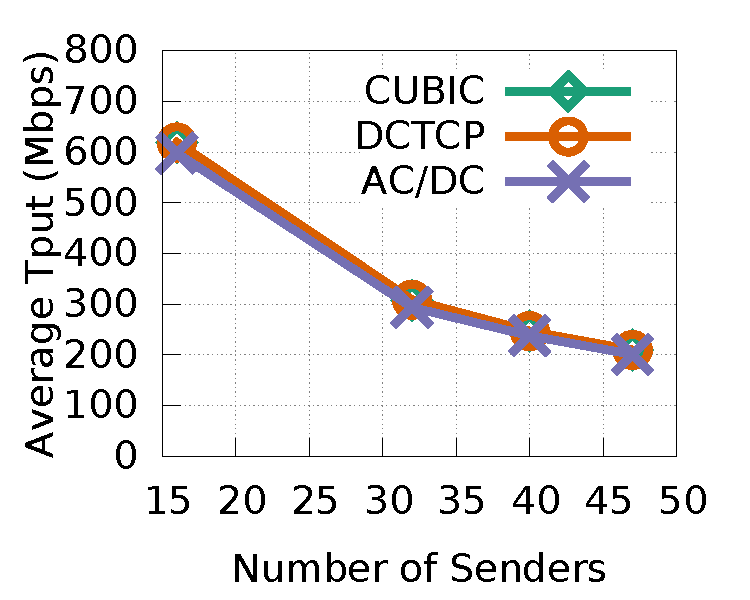
\includegraphics[width=\textwidth]{acdctcp/figures/incast/plots9k/incast_tput_vary_sender.pdf}
                \caption{Average throughput.}
                \label{incast_9k_tput}
        \end{subfigure}
        \begin{subfigure}[b]{0.45\textwidth}
                \centering
                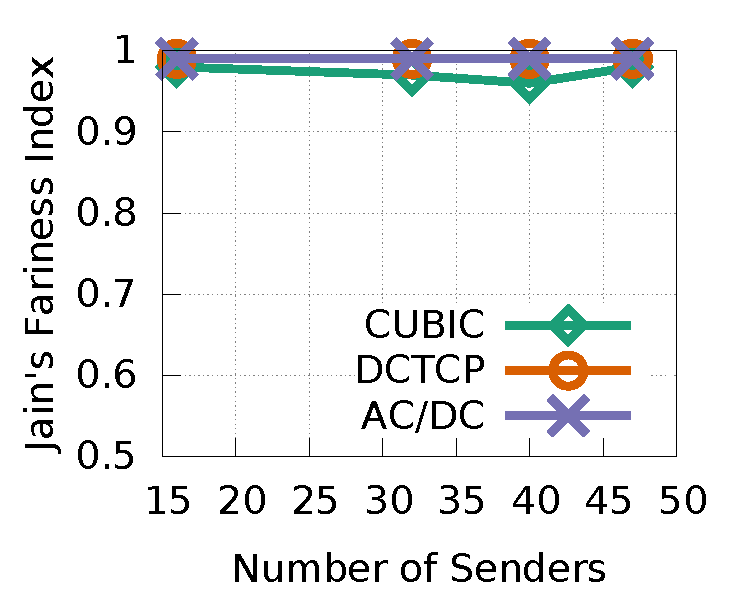
\includegraphics[width=\textwidth]{acdctcp/figures/incast/plots9k/incast_fairness_vary_sender.pdf}
                \caption{Fairness.}
                \label{incast_9k_fariness}
        \end{subfigure}
        \caption{Many to one incast: throughput and fairness.}
        \label{incast_9k_tput_fairness}
\end{figure}

\begin{figure*}[!t]
        \centering
        \begin{subfigure}[b]{0.45\textwidth}
                \centering
                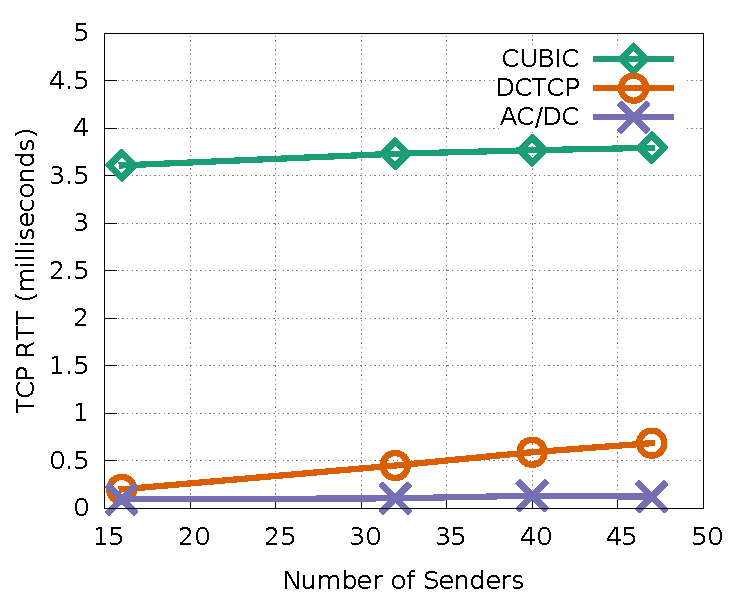
\includegraphics[width=\textwidth]{acdctcp/figures/incast/plots9k/incast_sockperf50th_vary_sender.pdf}
                \caption{50$^{th}$ percentile RTT.}
                \label{incast_9k_50th_sockperf}
        \end{subfigure}
        \begin{subfigure}[b]{0.45\textwidth}
                \centering
                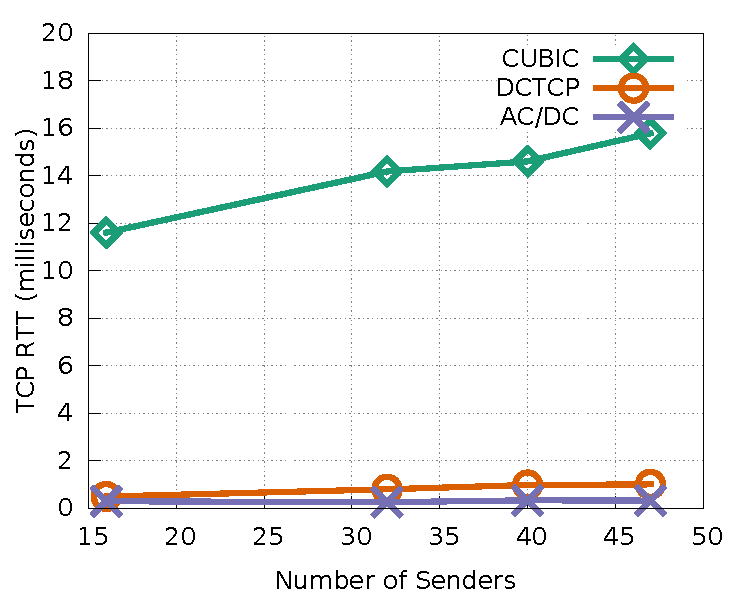
\includegraphics[width=\textwidth]{acdctcp/figures/incast/plots9k/incast_sockperf999th_vary_sender.pdf}
                \caption{99.9$^{th}$ percentile RTT.}
                \label{incast_9k_999th_sockperf}
        \end{subfigure}
        \begin{subfigure}[b]{0.45\textwidth}
                \centering
                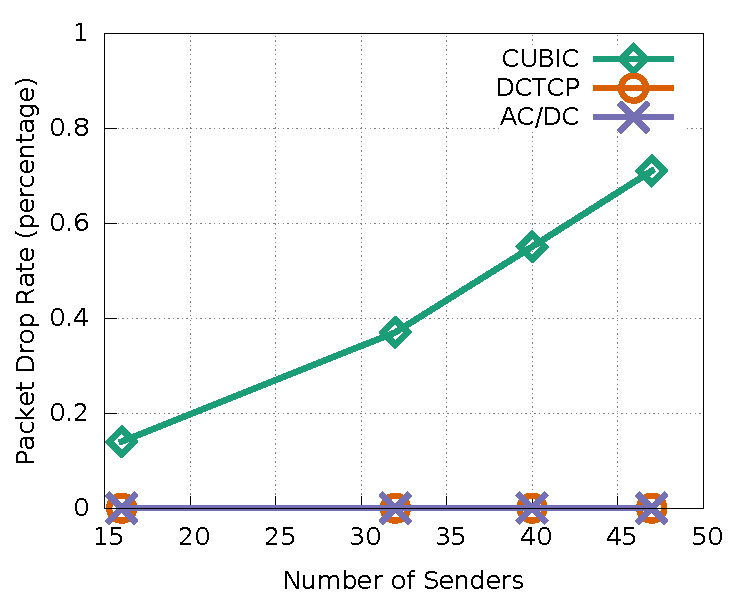
\includegraphics[width=\textwidth]{acdctcp/figures/incast/plots9k/incast_droprate_vary_sender.pdf}
                \caption{Packet drop rate.}
                \label{incast_9k_droprate}
        \end{subfigure}
        \caption{Many to one incast: RTT and packet drop rate.\crs{~\acdc{} can reduce DCTCP's RTT by limiting window sizes.}}
        \label{incast_9k_sockperf_droprate}
\end{figure*}


\begin{figure}[!t]
        \centering
  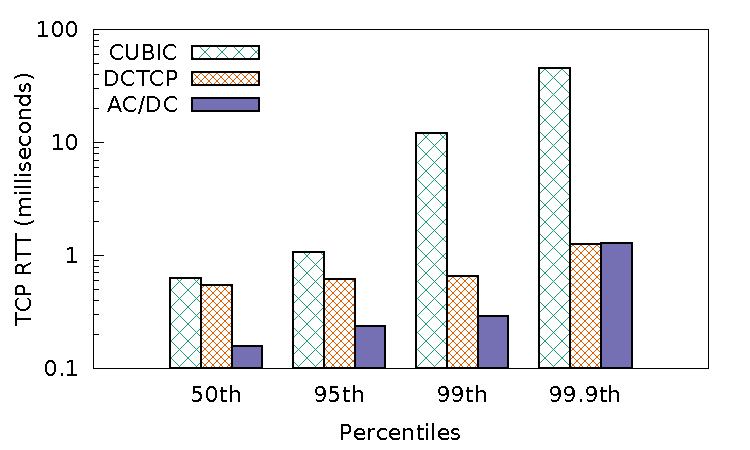
\includegraphics[width=0.7\textwidth]{acdctcp/figures/incast/pressure/incast_pressure_compare_sockperf.pdf}
        \caption{TCP RTT when almost all ports are congested.}
        \label{sockperf_pressure_incast}
\end{figure}



In this section we attach all servers to a single switch and
run a variety of workloads to better understand
how well~\acdc{} tracks DCTCP's performance. Experiments are run for 10 minutes. A simple TCP application
sends messages of specified sizes to measure FCTs.

\tightparagraph{Incast}
In this section, we evaluate incast scenarios.
To scale the experiment, 17 physical servers are equipped with four NICs each
and one flow is allocated per NIC.
In this way, incast can support up to 47-to-1 fan-in (our switch only has 48 ports).
We measure the extent of incast by increasing the number of concurrent senders to 16, 32, 40 and 47.
Figure~\ref{incast_9k_tput_fairness} shows throughput and fairness results.
Both DCTCP and \acdc{} obtain a fairness index greater than 0.99 and get comparable throughput as CUBIC.
Figure~\ref{incast_9k_sockperf_droprate} shows the RTT and packet drop rate results.
When there are 47 concurrent senders, DCTCP can reduce median RTT by 82\% and \acdc{} can reduce by 97\%;
DCTCP can reduce 99.9$^{th}$ percentile RTT by 94\% and \acdc{} can reduce by 98\%.
Both DCTCP and \acdc{} have 0\% packet drop rate. It is curious that~\acdc{}’s
performance is better than DCTCP when the number of senders increases (Figure~\ref{incast_9k_50th_sockperf}).
The Linux DCTCP code puts a lower bound of 2 packets on \cwnd{}.
In incast, we have up to 47 concurrent competing flows and
the network's MTU size is 9KB. In this case, the lower bound is too high,
so DCTCP's RTT increases gradually with the number of senders.
This issue was also found in~\cite{judd2015nsdi}.~\acdc{} controls \rwnd{} (which is in bytes)
instead of \cwnd{} (which is in packets) and \rwnd{}'s lowest value can be much smaller than 2*MSS.
We verified modifying~\acdc{}'s lower bound caused identical behavior.

\crs{The second test aims to put pressure on the switch's dynamic
buffer allocation scheme, similar to an experiment in the DCTCP paper~\cite{alizadeh2011data}.}
To this end, we aim to congest every switch port.
The 48 NICs are split into 2 groups: group $A$ and $B$.
Group $A$ has 46 NICs and $B$ has 2 (denoted $B_1$ and $B_2$).
Each of the 46 NICs in $A$ sends and receives 4 concurrent flows within $A$
(\ie{}, NIC $i$ sends to [$i+1$, $i+4$] mod 46).
Meanwhile, all of the NICs in $A$ send to $B_1$, creating a 46-to-1 incast.
This workload congests 47 out of 48 switch ports.
We measure the RTT between $B_2$ and $B_1$ (i.e., RTT of the traffic traversing the most congested port) and
the results are shown in Figure~\ref{sockperf_pressure_incast}.
The average throughputs for CUBIC, DCTCP, and~\acdc{} are 214, 214 and 201 Mbps respectively,
all with a fairness index greater than 0.98.
CUBIC has an average drop rate of 0.34\% but the most congested port has a drop rate as high as 4\%.
This is why the 99.9$^{th}$ percentile RTT for CUBIC is very high.
The packet drop rate for both DCTCP and~\acdc{} is 0\%.

\begin{figure*}[!t]
        \centering
        \begin{subfigure}[b]{0.7\textwidth}
                \centering
                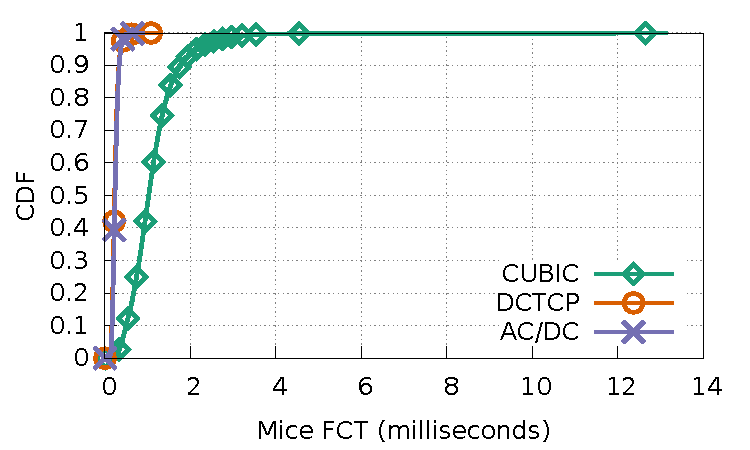
\includegraphics[width=\textwidth]{acdctcp/figures/macro_benchmarks/macro_4stride/stride4_mice16KB_fct.pdf}
                \caption{Mice flow completion times.}
                \label{macro_4stride_mice_fct}
        \end{subfigure}
        \begin{subfigure}[b]{0.7\textwidth}
                \centering
                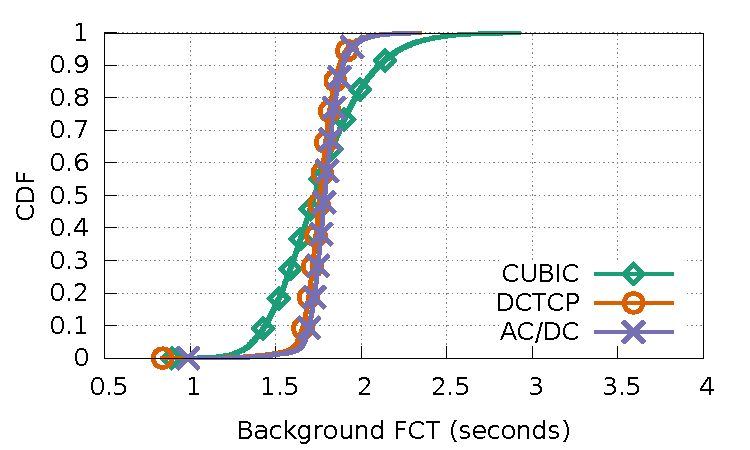
\includegraphics[width=\textwidth]{acdctcp/figures/macro_benchmarks/macro_4stride/stride4_big512MB_fct.pdf}
                \caption{Background flow completion times.}
                \label{macro_4stride_background_fct}
        \end{subfigure}
        \caption{CDF of mice and background FCTs in concurrent stride workload.}
        \label{macro_4stride_fct}
\end{figure*}

\begin{figure*}[!t]
        \centering
        \begin{subfigure}[b]{0.7\textwidth}
                \centering
                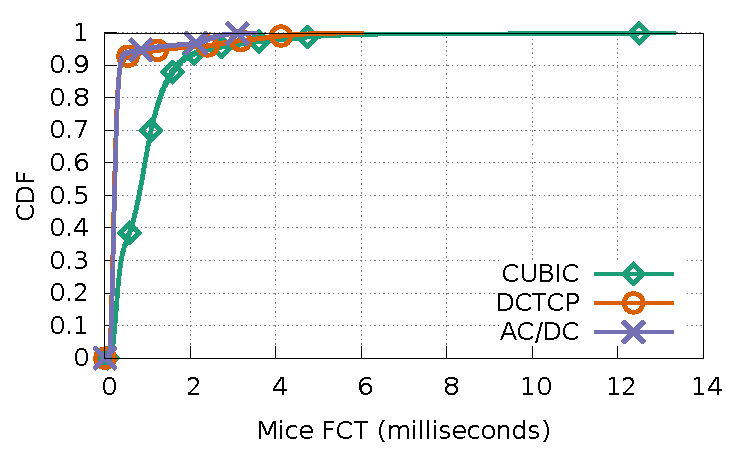
\includegraphics[width=\textwidth]{acdctcp/figures/macro_benchmarks/shuffle_17hosts/shuffle_mice16KB_fct.pdf}
                \caption{Mice flow completion times.}
                \label{macro_shuffle_mice_fct}
        \end{subfigure}
        \begin{subfigure}[b]{0.7\textwidth}
                \centering
                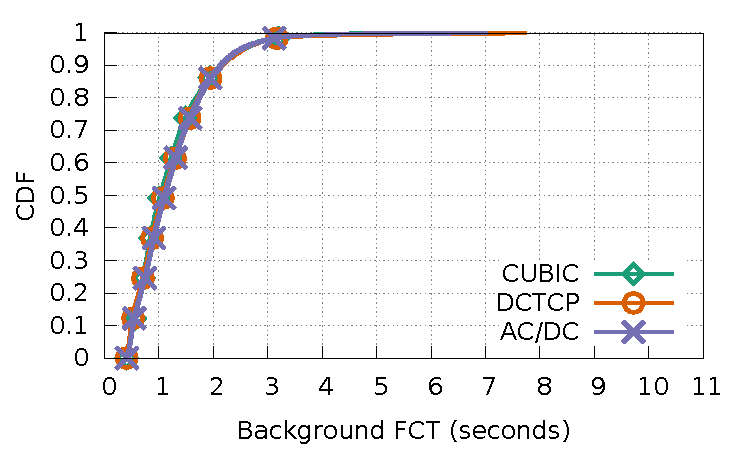
\includegraphics[width=\textwidth]{acdctcp/figures/macro_benchmarks/shuffle_17hosts/shuffle_big512MB_fct.pdf}
                \caption{Background flow completion times.}
                \label{macro_shuffle_background_fct}
        \end{subfigure}
        \caption{CDF of mice and background FCTs in shuffle workload.}
        \label{macro_shuffle_fct}
\end{figure*}

\begin{figure*}[!t]
        \centering
        \begin{subfigure}[b]{0.7\textwidth}
                \centering
                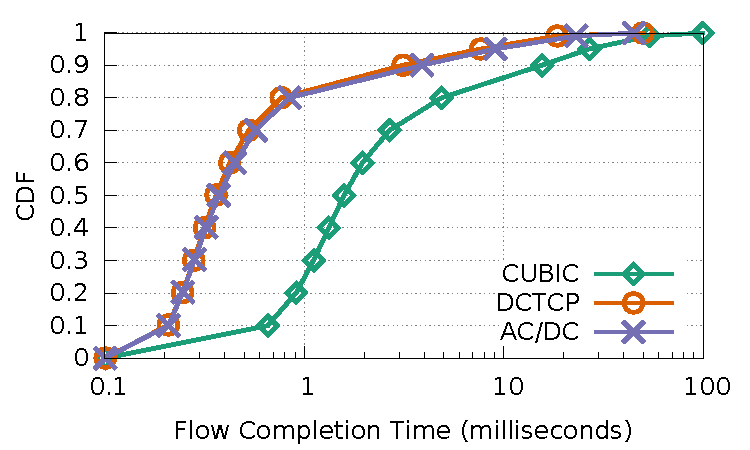
\includegraphics[width=\textwidth]{acdctcp/figures/macro_benchmarks/trace-driven/trace_driven_workload_dctcp_senders5_10points.pdf}
                \caption{Web-search workload.}
                \label{trace-driven-searching-fct}
        \end{subfigure}
        \begin{subfigure}[b]{0.7\textwidth}
                \centering
                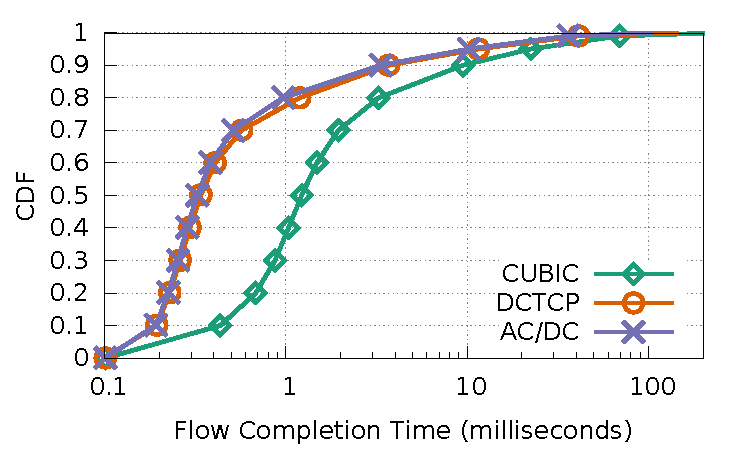
\includegraphics[width=\textwidth]{acdctcp/figures/macro_benchmarks/trace-driven/trace_driven_workload_conga_senders5_10points.pdf}
                \caption{Data-mining workload.}
                \label{trace-driven-data-mining-fct}
        \end{subfigure}
        \caption{CDF of mice (flows$<$10KB) FCT in web-search and data-mining workloads.}
        \label{macro-trace-driven-fct}
\end{figure*}

\tightparagraph{Concurrent stride workload}
In concurrent stride, 17 servers are attached to a single switch.
Each server $i$ sends a 512MB flow to servers [$i+1$, $i+4$] mod 17 in sequential fashion
to emulate background traffic.
Simultaneously, each server $i$ sends 16KB messages every 100 ms to 
server $(i+8)$ mod 17.
The FCT for small flows (16KB) and background flows (512MB) are shown 
in Figure~\ref{macro_4stride_fct}. For small flows, DCTCP and \acdc{} 
reduce the median FCT by 77\% and 76\% respectively. 
At the 99.9$^{th}$ percentile, DCTCP and \acdc{} reduce FCT by 91\% and 93\%, respectively.
For background flows, DCTCP and \acdc{} offer similar completion times.
CUBIC has longer background FCT because its fairness is not as 
good as DCTCP and \acdc{}.


\tightparagraph{Shuffle workload}
In shuffle, each server sends 512MB to every other server in random order. 
A sender sends at most 2 flows simultaneously and when
a transfer is finished, the next one is started until 
all transfers complete.
Every server $i$ also sends a 16 KB message to server $(i+8)$ mod 17 
every 100 ms. This workload is repeated for 30 runs.
The FCT for each type of flow is shown in Figure~\ref{macro_shuffle_fct}.
For small flows, DCTCP and \acdc{} reduce median FCT by
72\% and 71\% when compared to CUBIC. 
At the 99.9$^{th}$ percentile, DCTCP and \acdc{} 
reduce FCTs by 55\% and 73\% respectively.
For large flows, CUBIC, DCTCP and \acdc{} have almost identical performance.


\tightparagraph{Trace-driven workloads}
Finally, we run trace-driven workloads. 
An application on each server builds a long-lived TCP connection with every other server.
Message sizes are sampled from a trace and sent to a random destination in sequential fashion. Five
concurrent applications on each server are run to increase network load. Message
sizes are sampled from a web-search~\cite{alizadeh2011data}
and a data-mining workload~\cite{greenberg2009vl2,alizadeh2014conga}, whose flow size distribution has a heavier tail.
Figure~\ref{macro-trace-driven-fct} shows a CDF of FCTs for mice flows (smaller than 10KB) 
in the web-search and data-mining workloads.
In the web-search workload,
DCTCP and \acdc{} reduce median FCTs by 77\% and 76\%, respectively. 
At the 99.9$^{th}$ percentile, DCTCP and \acdc{} reduce FCTs by 50\% and 55\%, respectively.
In the data-mining workload, DCTCP and \acdc{} reduce median FCTs by 72\% and 73\%, respectively. 
At the 99.9$^{th}$ percentile, DCTCP and \acdc{} reduce FCTs by 36\% and 53\% respectively.  
%In both workloads, DCTCP and \acdc{} improve the fraction of mice flows that finish 
%in 1 millisecond significantly (from 20\%/30\% to 80\%).

\tightparagraph{Evaluation summary}
The results validate that congestion control can be accurately implemented in the vSwitch.
~\acdc{} tracks the performance of an unmodified host DCTCP stack
over a variety of workloads with little computational overhead.
Furthermore,~\acdc{} provides this functionality over 
various host TCP congestion control configurations. 
